\documentclass{article}

\usepackage{graphicx}
\usepackage{hyperref}
\usepackage{bm}
\usepackage{float}
\restylefloat{table}

\usepackage{listings}
\usepackage{color}
\usepackage{amsmath}

\usepackage[margin=1.25in]{geometry}

\definecolor{dkgreen}{rgb}{0,0.6,0}
\definecolor{gray}{rgb}{0.5,0.5,0.5}
\definecolor{mauve}{rgb}{0.86,0.27,0.22}

\lstset{frame=tb,
  language=python,
  aboveskip=3mm,
  belowskip=3mm,
  showstringspaces=false,
  columns=flexible,
  basicstyle={\small\ttfamily},
  numbers=none,
  numberstyle=\tiny\color{gray},
  keywordstyle=\color{blue},
  commentstyle=\color{dkgreen},
  stringstyle=\color{mauve},
  breaklines=true,
  breakatwhitespace=true,
  tabsize=3
}

%----------------------------------------------------------------------------------------
%	ASSIGNMENT INFORMATION
%----------------------------------------------------------------------------------------

\title{CS5200: Homework \#5} % Title of the assignment

\author{Matthew Whitesides\\ \texttt{mbwxd4@mst.edu}} % Author name and email address

\date{\today} % University, school and/or department name(s) and a date

%----------------------------------------------------------------------------------------

\begin{document}

  \maketitle % Print the title
 
  \begin{enumerate}
    \item \textbf{13.3-2 on p. 322.}
    
    So our goal is to insert and staisfy the cases:

    \begin{enumerate}
      \item All nodes are either red or black.
      \item Leaves are all black.
      \item Red nodes have black children.
      \item Equal number of black nodes in max paths.
      \item All internal nodes have two children – all leaves are NILs and are considered black.
    \end{enumerate}

    Our tree will be built like so {41, 38, 31, 12, 19, 8} (B = Black, R = Red):

    \begin{enumerate}
      \item Insert 41. Result: 41B.
      \item Insert 48. Result: 41B (left)$\rightarrow$ 38R.
      \item Insert 31. Result: 41B (left)$\rightarrow$ 38R (left)$\rightarrow$ 31R.
      \item Recolor 38R to 38B to staisfy case 3. Result: 41B (left)$\rightarrow$ 38B (left)$\rightarrow$ 31R.
      \item Recolor 41B to 41R to staisfy case 4. Result: 41R (left)$\rightarrow$ 38B (left)$\rightarrow$ 31R.
      \item Rotate to the right to balance the tree on 38. Result:\\
      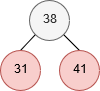
\includegraphics[scale=0.5]{1a.png}
      \item Insert 12 to the left of 31 to result in 12R.
      \item Recolor 31, 41 and 38 to black to keep case 3. Result:\\
      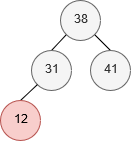
\includegraphics[scale=0.5]{1b.png}
      \item Insert 19R to the right of 12R. 
      \item Rotate left on 12R to put 19R above 12R.
      \item Rotate right on 19R to balance and put 12R and 31 below 19R.
      \item Recolor 19R to black to staisfy caes 4. Result:\\
      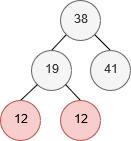
\includegraphics[scale=0.5]{1c.png}
      \item Insert 8R to the left of 12R.
      \item Recolor 12R and 31R to black, and recolor 19B to red to satisfy case 4. Final Result:\\
      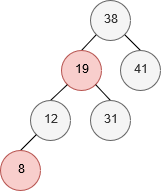
\includegraphics[scale=0.5]{1d.png}

    \end{enumerate}

    \item \textbf{13.4-3 on p. 330.}
    
    Remove {8, 12, 19, 31, 38, 41}:

    \begin{enumerate}
      \item Remove 8:\\
      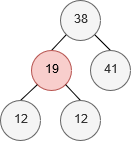
\includegraphics[scale=0.5]{2a.png}
      \item Remove 12.
      \item Recolor 19 to black.\\
      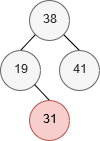
\includegraphics[scale=0.5]{2b.png}
      \item Rotate 19 right to put 31 above 19.
      \item Remove 19.\\
      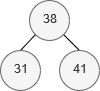
\includegraphics[scale=0.5]{2c.png}
      \item Recolor 31 and 41 to red.
      \item Remove 31.\\
      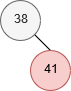
\includegraphics[scale=0.5]{2d.png}
      \item Remove 41.\\
      
\includegraphics[scale=0.5]{2e.png}
      \item Finally remove 38.
    \end{enumerate}

    \item \textbf{15.2-2 on p. 378. Implement your algorithm.}
    
    TODO!!!!!

    \item \textbf{15.4-1 on p. 396.}
    
    The longest common subsequence of $\left\{ 1, 0, 0, 1, 0, 1, 0, 1 \right\}$ and $\left\{ 0, 1, 0, 1, 1, 0, 1, 1, 0 \right\}$ would be \bm{$\left\{ 1, 0, 0, 1, 1, 0 \right\}$}.
    
    Note however there could be more than one of this length.

    You could find this using an iterative substring algorithm like so:

    \begin{lstlisting}
      def lcs(s1, s2):
      table = [["" for x in range(len(s2))] for x in range(len(s1))]
      for i in range(len(s1)):
          for j in range(len(s2)):
              if s1[i] == s2[j]:
                  if i == 0 or j == 0:
                      table[i][j] = s1[i]
                  else:
                      table[i][j] = table[i-1][j-1] + s1[i]
              else:
                  table[i][j] = max(table[i-1][j], table[i][j-1], key=len)
      return table[-1][-1]

      print(lcs("10010101", "010110110"));

      #Output: 100110
    \end{lstlisting}

    \item \textbf{15.4-5 on p. 397.}
    
    To find the longest monotonically increasing sub-sequence of a sequence of n numbers, in $O(n^2)$ time would go something like so:

    \begin{enumerate}
      \item Let $S\;=\;a\;sequence\;of\;n\;numbers$.
      \item Let $LMIS\;of\;S\;=\;Longest\;Monotonically\;Increasing\;Sub Sequence\;of\;S$.
      \item For $i\;in\;range(n)$ let Monotonically increasing sub sequence $mis(i)$ be the length of the longest $mis(i)$ for $sequence s\;in\;s_1, s_2, ... s_i$.
      \item Thus we seek the max length of the sequence $mis(i) \in i \in range(n)$.
      \item We'll want to find the LMIS of each MIS(i) and fill in a table of each value, then find the longest value in the table to find the LMIS(n).
      \item To find the MIS(i) recursively go trough to find the $LMIS(s_{i - 1})$ until you hit the base case of i = 1 which the LMIS of a sequence of one is the element itself. 
      \item Then for each other case check (lets call the recursive call iteration $j$) if $j \leq i -1$ you keep going otherwise return to finish the recursion. 
      \item Once you have finished for each sub sequence $s$ in $S$ you scan the table for the longest value.
      \item The recusive part to fill the table would take $O(n^2)$ time and the part to find the max value in the table would take $O(n)$ time giving a total of $O(n^2)$.
    \end{enumerate}

    \item \textbf{16.1-3 on p. 422.}
    
    \begin{itemize}
      \item Show that the approach of selecting the activity of least duration from among those that are compatible with previously selected activities does not work.
      \begin{itemize}
        \item Say we have the following start and finsih times.
          \begin{table}[H]
            \centering
            \begin{tabular}{|l|lll}
            \hline
            $i$   & \multicolumn{1}{l|}{1} & \multicolumn{1}{l|}{2} & \multicolumn{1}{l|}{3} \\ \hline
            $s_i$ & 0                      & 4                      & 6                      \\ \cline{1-1}
            $f_i$ & 5                      & 7                      & 10                     \\ \cline{1-1}
            \end{tabular}
          \end{table}
        \item Using greedy we'd pick 4 - 7 first as it's the shortest length however since it overlaps with both column 1 and 3 we'd eliminate both those, however they don't overlap eachother so we could have had two periods instead of just the one.
      \end{itemize}
      \item Do the same for the approaches of always selecting the compatible activity that overlaps the fewest other remaining activities.
      \begin{itemize}
        \item Say we have the following table.
        
        \begin{table}[H]
          \centering
          \begin{tabular}{|l|lllllllllll}
          \hline
          $i$   & \multicolumn{1}{l|}{1} & \multicolumn{1}{l|}{2} & \multicolumn{1}{l|}{3} & \multicolumn{1}{l|}{4} & \multicolumn{1}{l|}{5} & \multicolumn{1}{l|}{6} & \multicolumn{1}{l|}{7} & \multicolumn{1}{l|}{8} & \multicolumn{1}{l|}{9} & \multicolumn{1}{l|}{10} & \multicolumn{1}{l|}{11} \\ \hline
          $s_i$ & 0                      & 1                      & 1                      & 1                      & 3                      & 5                      & 7                      & 9                      & 9                      & 9                       & 11                      \\ \cline{1-1}
          $f_i$ & 2                      & 4                      & 4                      & 4                      & 6                      & 8                      & 10                     & 12                     & 12                     & 12                      & 13                      \\ \cline{1-1}
          \end{tabular}
        \end{table}

        \item Essentailly this is the easist thing I could think of you have everything but the middle column with three conflicts where i=6 has two. That would give you columns 6,1,8 using greedy lest conflicts however a more optimal solution would be columns 1,5,7,11.
      \end{itemize}
      \item And for always selecting the compatible remaining activity with the earliest start time.
      \begin{itemize}
        \item Say we have the following table.
        \begin{table}[H]
          \centering
          \begin{tabular}{|l|lll}
          \hline
          $i$   & \multicolumn{1}{l|}{1} & \multicolumn{1}{l|}{2} & \multicolumn{1}{l|}{3} \\ \hline
          $s_i$ & 0                      & 1                      & 6                      \\ \cline{1-1}
          $f_i$ & 7                      & 5                      & 10                     \\ \cline{1-1}
          \end{tabular}
        \end{table}
        \item Here we'd instantly pick column 1 and only have one period insead of being able to fit in two if we went with columns 2 \& 3.
      \end{itemize}
    \end{itemize}

    \item \textbf{16.2-5 on p. 428.}
    
    Given we're talking about greedy algorithms in the chapter I figure we'll try to set up one of those to get an optimal smallest set of closed intervals that contains all the given points.
    Also we're going to assume that unit-length can be determined by adding 1 to a value.

    \begin{enumerate}
      \item Initially define out initial set as $X$ and our solution set as $S = {}$.
      \item First sort the points in set $X$ by value so they are monotonically increasing in order $x_1, x_2,...x_n$.
      \item Set $S = \{[x_0, x_0 + 1]\}$. // The first interval will be the smallest unit plus 1.
      \item For $x_i \in X[1:]$: // For each element in set X starting at the second point.
      \begin{itemize}
        \item If $x_i \notin max(S)$ then: // If current iteration of X is not contained in the previsouly added interval.
        \begin{itemize}          
          \item $S = S \cup [x_i, x_i + 1]$ // Append interval made from current x and x + 1.        
        \end{itemize}
        \item Return $S$.
      \end{itemize}
    \end{enumerate}

    We can argue this will always produce an optimal set given that the largest element must be containted in the [largest x, largest x + 1] and recursivly you could go through each element and compare it plus one unit to each other element to produce a set.
    Therefore this solution must be optimal as no element in the set could be outside the sorted max and min and each element is given an interval if the previous intervals do not contain it.
    The efficiency of the alogrithm would be pretty much as fast as the sorting would take (unless somehow the sorting was less than O(n)) which would probably be O(n log n) if using a quick sort like method.

    \item \textbf{16.3-3 on p. 436.}
    
    Given how the Huffman coding creates the tree you can pretty easily conceptualize how this will work. 
    \begin{itemize}
      \item Since we have an exponentially increasing sequence the coding will start with a \& b create a tree with node 2 as the root and a \& b as children.
      \item Next It'll append the sum of the root (which remeber is the sum of the first two numbers 2) and add node c to that which is 2 as well giving 4. Since 2 is less than 4 it'll be the left node.
      \item Next it'll do the same 4+3 = 7 and since 3 is less it'll be the left node.
      \item And so on and so on, the sum node will always be incresing faster then the fib numbers themselves so we'll continually get one level deeper and to the left for every fib number except the first two.      
    \end{itemize}

    Therefore the patten to generallize for any n fib numbers would just be starting at the column(n) you have 0 then add a 1 in front for each decending column until you get to the last node with would not add a 1 it would just change the 0 to a 1.

    \begin{table}[H]
      \centering
      \begin{tabular}{|l|llllllll}
      \hline
                & \multicolumn{1}{l|}{a} & \multicolumn{1}{l|}{b} & \multicolumn{1}{l|}{c} & \multicolumn{1}{l|}{d} & \multicolumn{1}{l|}{e} & \multicolumn{1}{l|}{f} & \multicolumn{1}{l|}{g} & \multicolumn{1}{l|}{h} \\ \hline
      Frequency & 1                      & 1                      & 2                      & 3                      & 5                      & 8                      & 13                     & 21                     \\ \cline{1-1}
      codeword  & 1111110                & 1111111                & 111110                 & 11110                  & 1110                   & 110                    & 10                     & 0                      \\ \cline{1-1}
      \end{tabular}
      \end{table}

    \item \textbf{17.4-3 on p. 471.} 
    
    To do a simmular analysis of the cost of the $i^{th}$ table insert using an expansion at $\frac{2}{3}$ instead of $\frac{1}{2}$, we'll start with if the $i^{th}$ operation does not trigger an expansion.

    This will actually be the same as for half considering that it only costs $c_i = 1$ for deleting one element, so according to the book page 466 we'll have.

    \[\hat{c} = c_i + \phi_i + \phi_{i - 1} = 3\]

    Now the real question is what happens when we use up $\frac{2}{3}$ of our data then what is the cost. Remember $c_i = num_i + 1$, and we have $size_i = size_{i-1}/3$, $size_{i-1} = 3num_{i - 1}$ and  $num_{i-1} = num_i + 1$. 
    Therefore the amortized cost of the operation is using out potential function $|2 \cdot T.num - T.size|$:

    \[\hat{c_i} = c_i + \phi_i - \phi_{i-1}\]
    \[=(num_i + 1) + (size_{i-1}/3 - 2num_i) - (size_{i-1}/3 - 2num_{i-1}) \]
    \[= 2\]

    \[\hat{c} = c_i + \phi_i + \phi_{i - 1}\]
    \[= (num_i + 1) + |(2num_i - size_i)| - |(2num_{i - 1} - size_{i - 1})|\]
    \[= (num_i + 1) + |(2num_i - 2(num_i + 1))| - |(2(num_i + 1) - 3(num_i + 1)|\]
    \[= 3\]

    Meaning that we are still bound by at most a constant factor of 3.

    \item \textbf{18.2-1 on p. 497.}
    
    Insert keys, $\{F, S, Q, K, C, L, H, T, V, W, M, R, N, P, A, B, X, Y, D, Z, E\}$.
    I'm thinking showing the graph before a split as I draw the graph then the next action causes the split wich I'll spell out.

    \begin{enumerate}
      \item First inset F, S and the median key Q.\\
      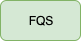
\includegraphics[scale=0.5]{10a.png}
      \item Insert K splitting up PQS.
      \item Then insert C to the left using F as the new median.\\
      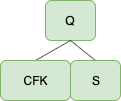
\includegraphics[scale=0.5]{10b.png}
      \item We can insert L to the left, making that node large then (2t - 1) so it must split on F which gets promoted.
      \item Insert H, T, V into their respective order.\\
      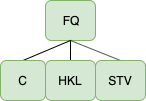
\includegraphics[scale=0.5]{10c.png}
      \item Insert W which causes STV to split and promote T.\\
      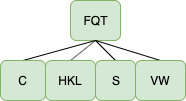
\includegraphics[scale=0.5]{10d.png}
      \item Insert R which causes HKL to split then cuases FQT to split creating a new root Q.
      \item Then Insert M, N.\\
      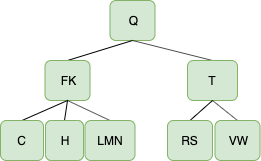
\includegraphics[scale=0.5]{10e.png}
      \item Insert P which causes LMN to split.
      \item Then Insert A, B, X.\\
      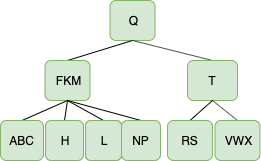
\includegraphics[scale=0.5]{10f.png}
      \item Insert Y which causes VWX to split.\\
      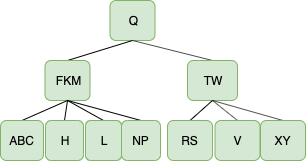
\includegraphics[scale=0.5]{10g.png}
      \item Insert D which causes ABC to split then FKM to split.
      \item And Finally insert Z,E.\\
      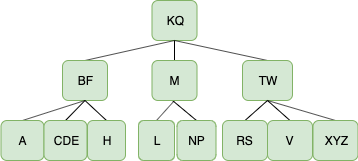
\includegraphics[scale=0.5]{10h.png}
    \end{enumerate}

    \item \textbf{18.3-1 on p. 502.}
    
    Delete ${C, P, V}$ from B-Tree 18.8(f).
    
    \begin{enumerate}
      \item Initial Tree.\\
      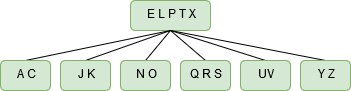
\includegraphics[scale=0.5]{11a.png}
      \item Delete C, case 2b (Merge AE and JK to satisfy the root having n + 1 children).\\
      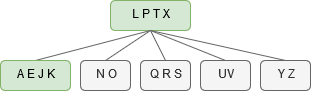
\includegraphics[scale=0.5]{11b.png}
      \item Delete P, case 3b.\\
      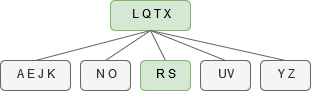
\includegraphics[scale=0.5]{11c.png}
      \item Delete C, case 2b.\\
      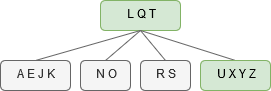
\includegraphics[scale=0.5]{11d.png}            
    \end{enumerate}

    \item \textbf{19.2-1 on p. 518.}
    
    So the minimum node we're going to extract is node 7.\\
    Which starts simply enough we'll remove 7 and add 17, 23, 24 up to the root list.\\
    Then the consolidation occurs which means 24 and 18 merge will merge, and 17 and 38 merge as they have the same order.\\
    Giving us the final result.\\

    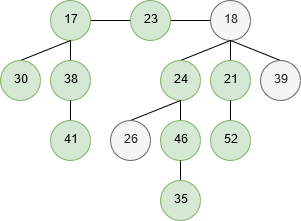
\includegraphics[scale=0.75]{12.png}

    \item \textbf{19.4-1 on p. 526.}
    
    We'll attempt to prove that a Fibonacci Heap does not always have a height $O(log\;n)$ by showing the sequence of operations creating a Fib Heap of one tree that is a linear chain of $n$ nodes.

    The basic steps for inserting into a Fibonacci heap are:

    \begin{enumerate}
      \item Initialize node $x$.
      \item Test if Fib heap $H$ is empty. 
      \begin{itemize}
        \item If so make $x$ the only node in the root list and set $H.min$ to $x$.
        \item Else inset $x$ into the $H$ root list and update $H.min$ if $x$ is smaller than it.
      \end{itemize}
      \item Increment $H.n$ if nesscary.
    \end{enumerate}

    We can use this to determine the idea of how we can create a heap with our desiered linear property. Think of the following steps.

    \begin{enumerate}
      \item Start with an empty set $H$, add three nodes from smallest to largest $x, y, z$ this makes $H.min = x$.
      \item Delete node $x$ which will call Extract min and consolidate and thus linking $y$ and $z$ with y being the new $H.min = y$.
      \item Lets define this new tree as $T$ which is just a linking of $y -> z$. 
      \item Now do the same thing with three new nodes in increasing value order $x_i, y_i, z_i$. (now we have four trees $y -> z$, $x_i$, $y_i$, $z_i$).
      \item Delete the smallest value $x_i$. which will link $y_i -> z_i$ and $y$ will link with $y_i$. Giving somthing like:\\
      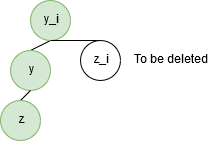
\includegraphics[scale=0.5]{13.png}     
      \item Now just delete $z_i$ and you have a single connected list of nodes.
      \item Just repet the previous 3 steps for more decreaseing values of $x_i, y_i, z_i$ and you can indefinately create a single list.
    \end{enumerate}

    This makes since as you always are deleting the min of your new set, creating a node with one link, mergeing into your existing set and deleting the linked node from your new set thus adding only one node to the merged set at the end.

    \item \textbf{21.3-2 on p. 572. Implement your algorithm.}
  \end{enumerate}

\end{document}
